\chapter{Esperimenti Localizzazione}\label{ch:chapter2}
In questo capitolo si andrà a descrivere il lavoro effettuato per estrarre le azioni di nostro interesse dall'intero video delle partite presente nel nostro test set.
\\Per fare ciò abbiamo utilizzato la rete neurale addestrata nel problema di classificazione descritto precedentemente.
\\Quello che abbiamo fatto  può sembrare stano, infatti abbiamo trasformato un problema di \textbf{classificazione} in uno di \textbf{localizzazione}, tuttavia vedremo che nel nostro caso, con qualche accorgimento, ciò è realizzabile.
\section{Sliding windows dataset}
Il Dataset su cui andremo a effettuare la localizzazione è ovviamente il test set del problema precedente (non avrebbe senso cercare di localizzare azioni in porzioni di dataset utilizzate per il training).
\\Tuttavia, se nel caso precedente avevamo diviso ogni partita del dataset in porzioni \textbf{disgiunte} di un minuto, nel caso della localizzazione ciò non è ovviamente utile ai nostri scopi.
\\Un altro fattore da considerare, se come detto si vuole utilizzare la rete neurale precentemente addestrata, è  il tipo di dati forniti in fase di training a tale rete: \textbf{120} raggruppamenti di features (ovvero un \textbf{minuto} di video) per ogni campione.
\\Per queste motivazioni, partendo dalle features estratte dall'intero video, è stato creato un campione per ogni secondo di partita, sempre formato da 120 raggruppamenti di features, mediante un meccasismo di \textbf{sliding windows}.
\\Più nel dettaglio il campione corrsipondente all'istante di partita \textbf{t} viene creato in modo da contenere tutte le features dei frame dall'istante \textbf{t-30} all'istante \textbf{t+30}.
\\Ad esempio il campione corrispondente al minuto di partita 23,57 sarà formato dalle features dei frame comprese tra il minuto 23,27 e il minuto  24,27.
\\Ovviamente per i campioni all'\textbf{inizio} e alla \textbf{fine} della partita, ovvero i campioni corrispondenti ai primi 30 secondi di video e quelli corrispondenti agli ultimi 30, si sono dovuti prendere degli accorgimenti dato che la loro finestra di features \textit{usciva dal video}. Per questo motivo al posto delle features mancanti sono state inserite delle features \textbf{fittizie}, tutte poste a \textbf{zero}, per consentire il corretto funzionamento della rete neurale.
\\Questa costruzione del dataset permette di utilizzare la rete neurale precedentemente addestrata per i nostri scopi di \textbf{localizzazione}.
\section{Predizioni}
Una volta processato il test set come sopra descritto, mediante quindi un meccanismo di sliding windows, è stato utlizzato il metodo \textbf{predict} fornitoci dalla libreria keras \cite{chollet2015keras}, il quale dato un modello già alleneato e dei dati compatibili con tale modello, ci fornisce in output le sue predizioni su tali dati sotto forma di probabilità. 
\\Per esempio nel nostro caso, ad ogni \textbf{campione}, quindi ad ogni \textbf{secondo} di partita, sono assegnate \textbf{quattro} probabilità, ovvero una per ogni label (background, sostituzione, cartellino, goal).
\\Ovviamente per come abbiamo costruito il nostro dataset, le probabilità di un evento ad un certo istante di tempo si riferisce al fatto che sia presente o meno tale evento nei trenta secondi \textbf{precedenti} o nei trenta secondi \textbf{successivi} al nostro tempo di riferimento.
\\Questo processo è stato ripetuto poi per tutte le partite del nostro test set.
\begin{figure}[ht]
\centering
\caption{Rappresentazione grafica delle predizioni}
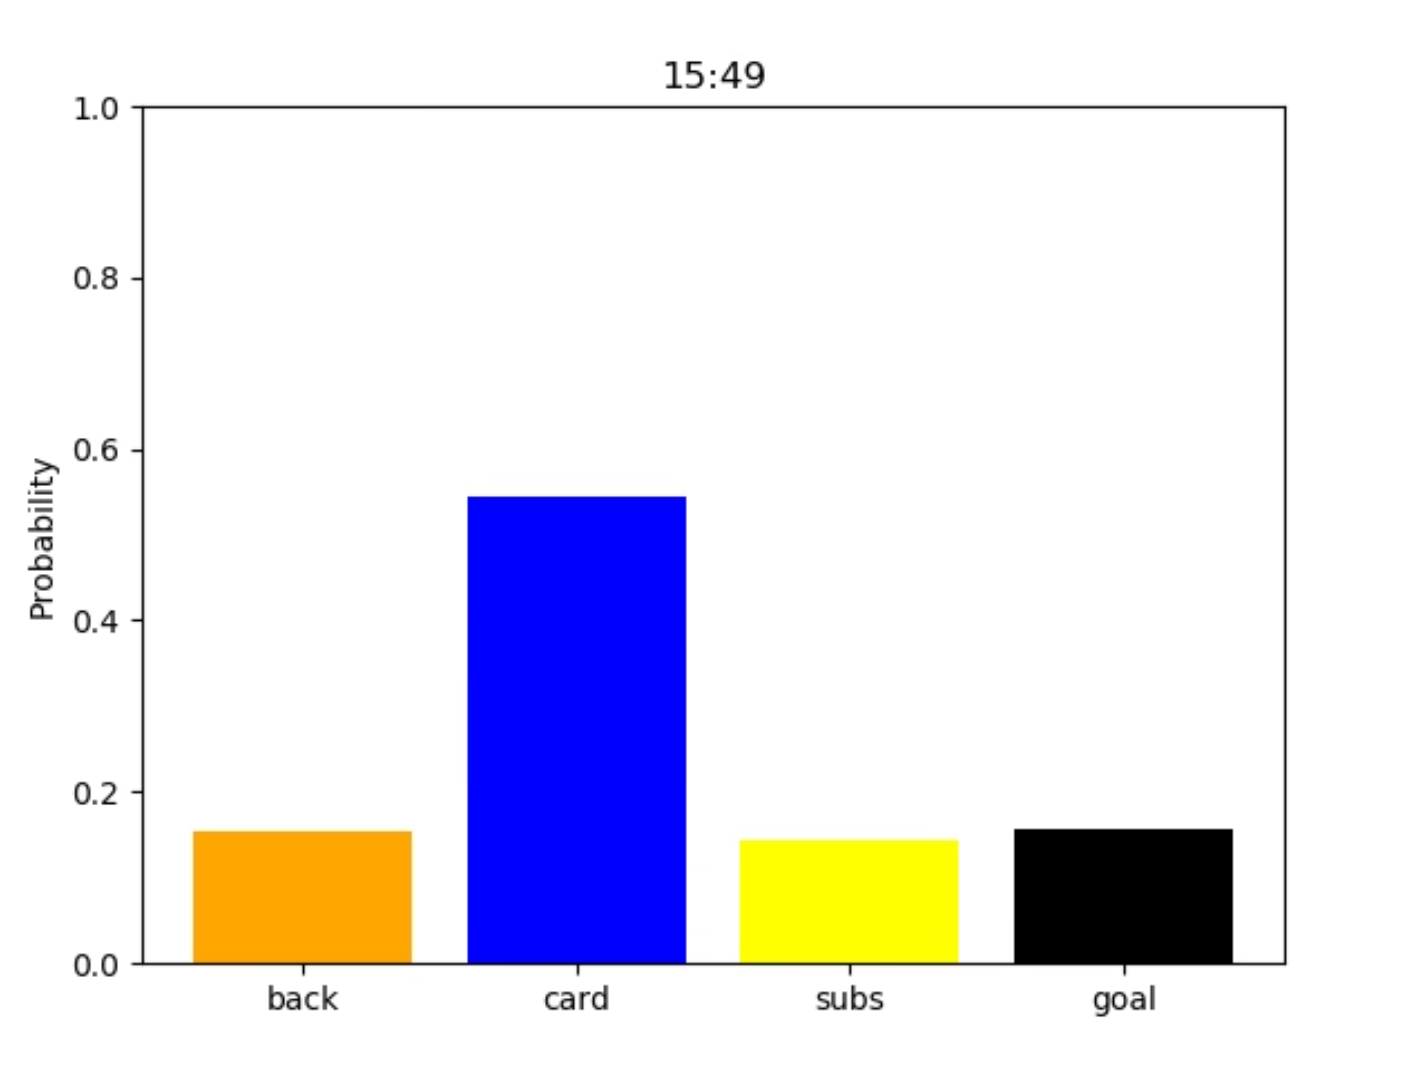
\includegraphics[width=\linewidth]{img/predict.png}
\label{figure : predict}
\end{figure}
\section{Visualizzazione predizioni}
Per verificare il corretto funzionamento del mio modello anche nel task di localizzazione, con l'ausilio delle librerie \textbf{matplotlib} e \textbf{OpenCV}, sono stato in grado di mostare direttamente le predizioni (in tempo reale) sopra il video della partita.
\\Questo ci ha permesso di comprendere molto meglio gli aspetti che la rete neurale ritiene importanti e che fanno la differenza tra un campione con la label di \textit{background} e un campione con una label più significativa.

\begin{figure}[ht]
\centering
\caption{Visualizzazione di un goal correttamente predetto}
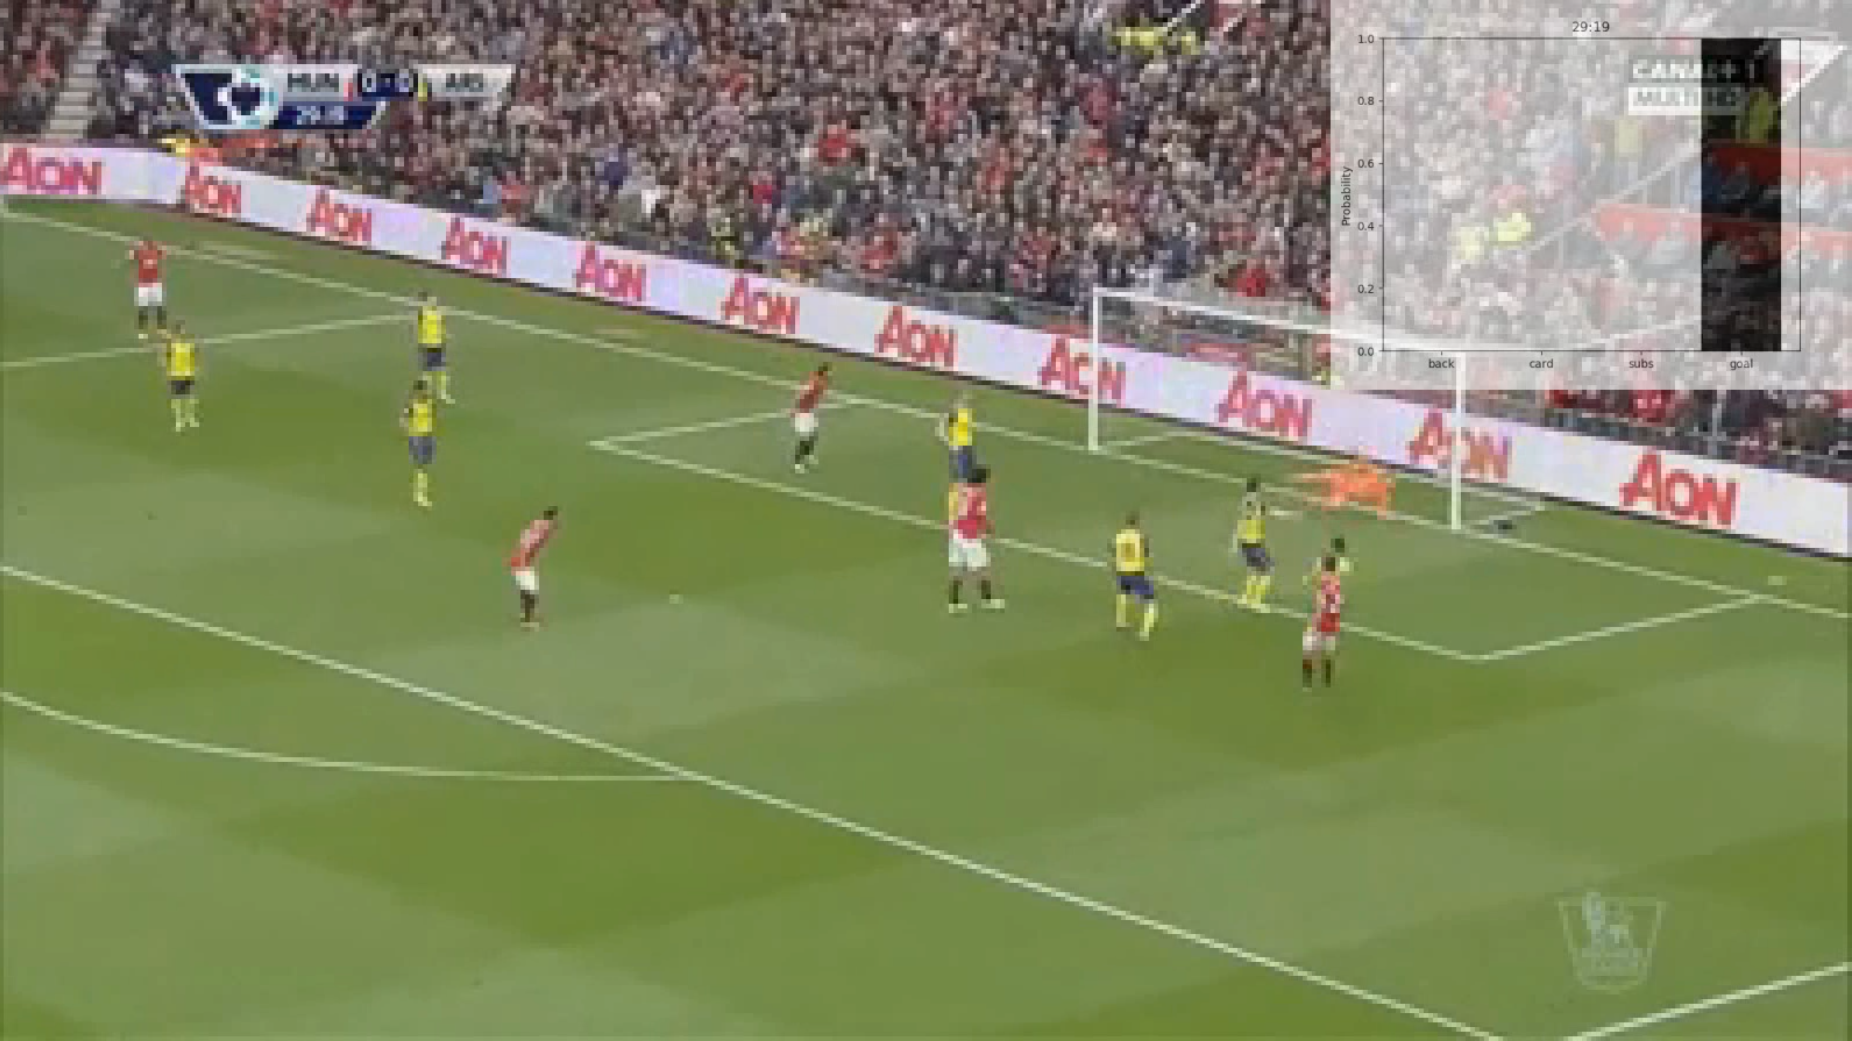
\includegraphics[width=\linewidth]{img/videogoal.png}
\label{figure : videogoal}
\end{figure}
\begin{figure}[H]
\centering
\caption{Visualizzazione di un cartellino correttamente predetto}
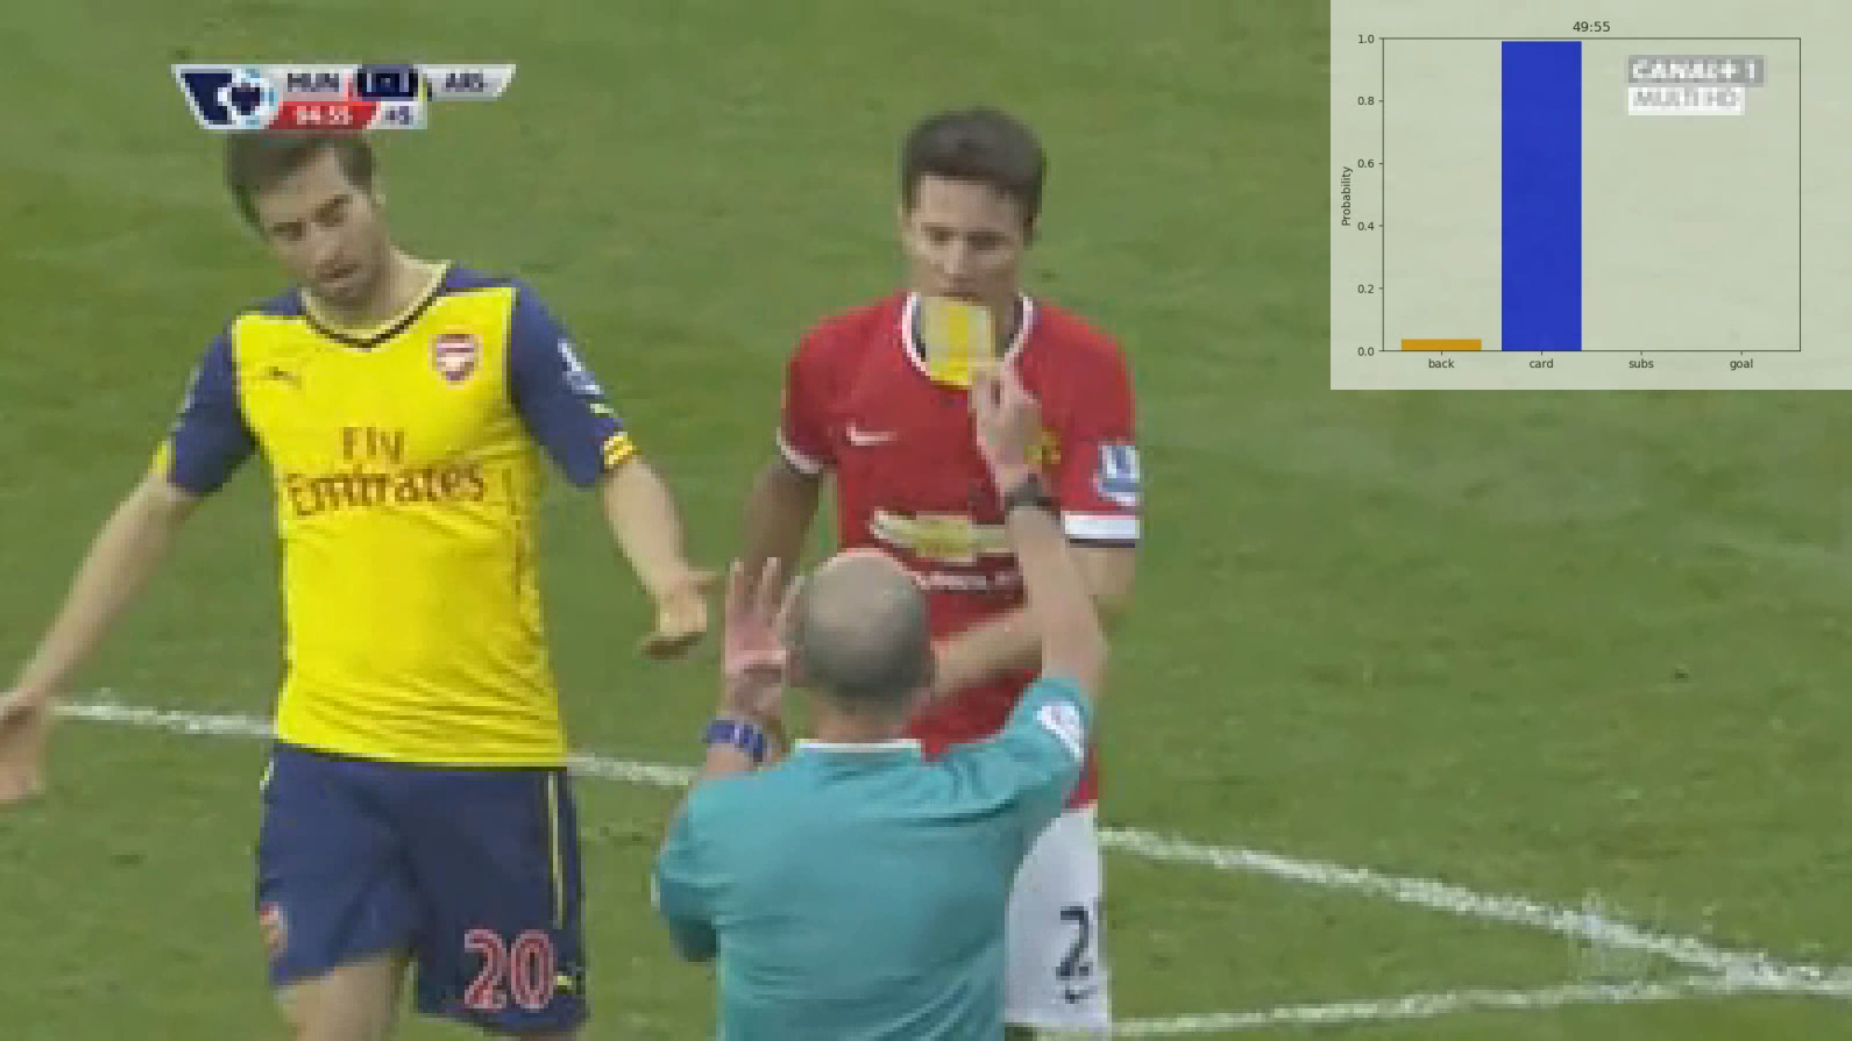
\includegraphics[width=\linewidth]{img/videocard.png}
\label{figure : videocard}
\end{figure}
\begin{figure}[H]
\centering
\caption{Visualizzazione di un sostituzione correttamente predetta}
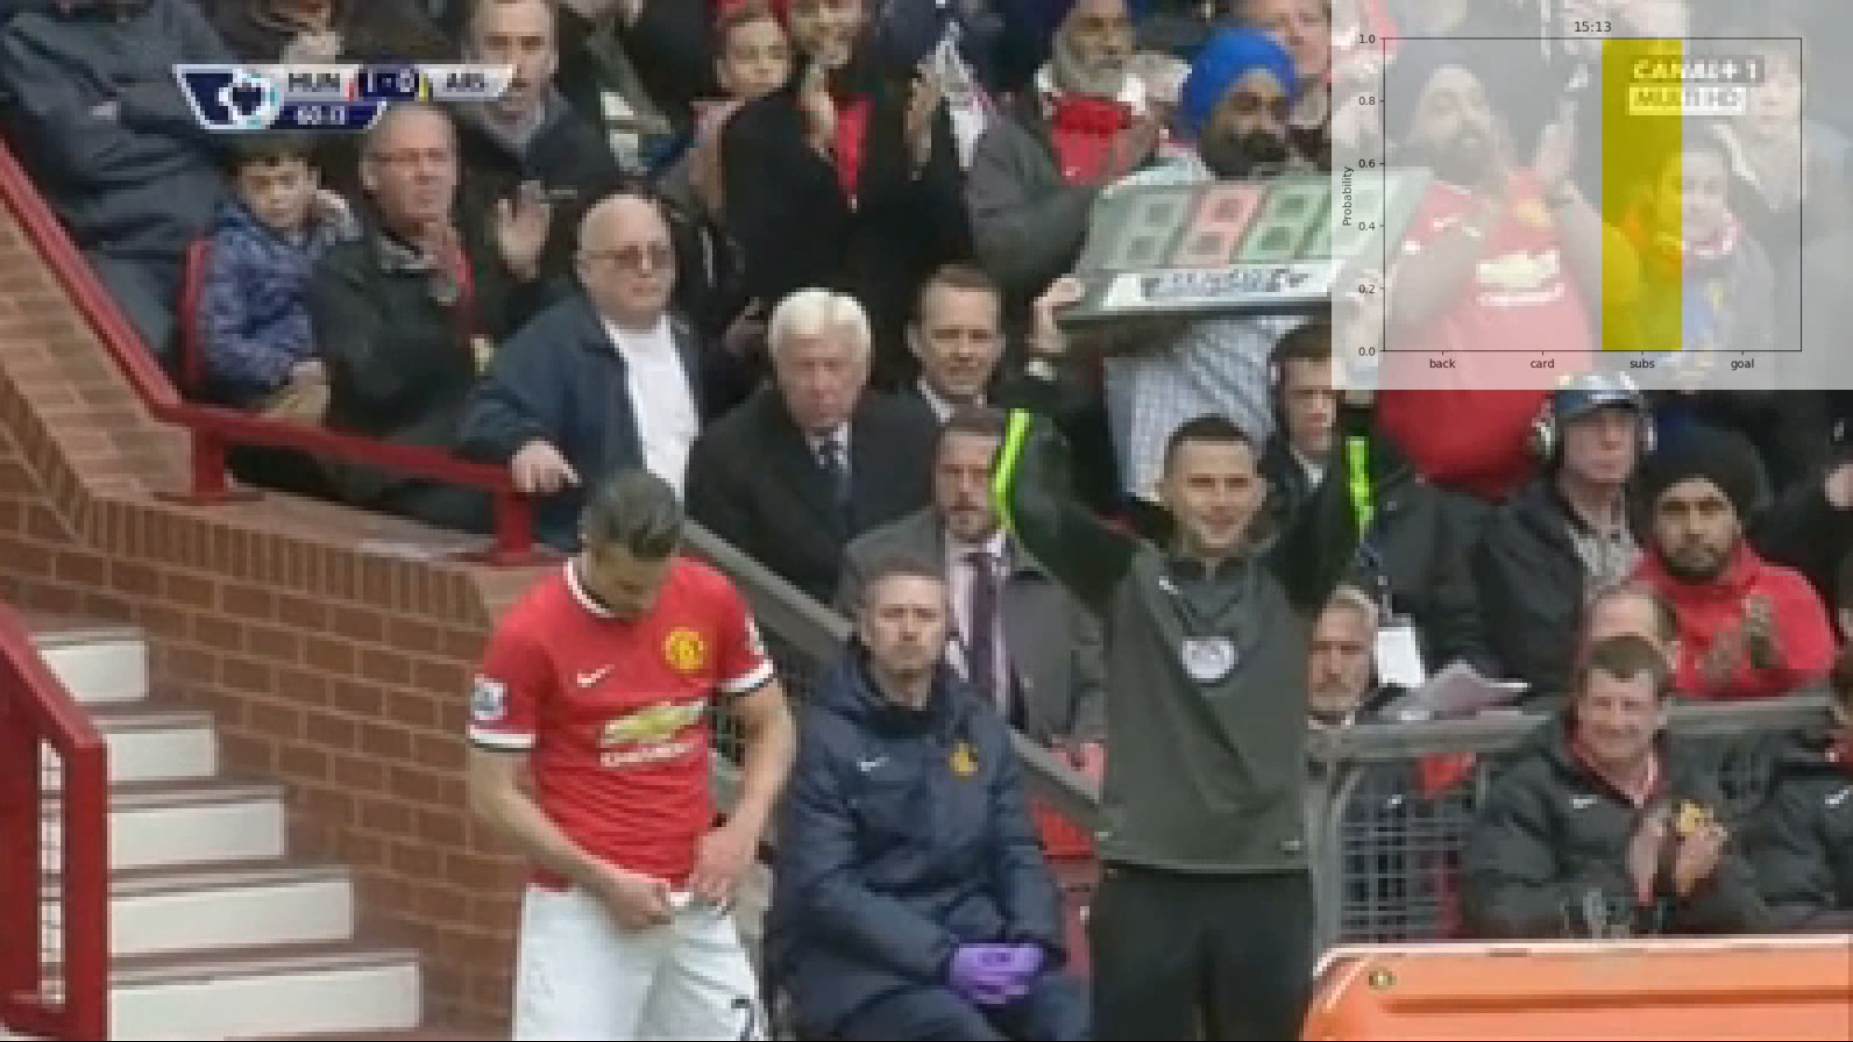
\includegraphics[width=\linewidth]{img/videosubs.png}
\label{figure : videosub}
\end{figure}
\section{Highlighs}
Dopo aver generato le predizioni, si ha quindi per ogni istante di una partita la probabilità che i tre nostri eventi di riferimento siano vicini a tale istante.
\\Prima di procedere con la generazione degli highlights, tuttavia è necessario determinare alcuni parametri:
\begin{itemize}
\item La \textbf{probabilità di soglia}, ovvero la probabilità minima che il campione deve avere per ritenerlo appartente ad un azione da noi ricercata. Di default tale valore è impostato a \textbf{0.9} in quanto il modello da noi trovato fornisce predizioni molto polarizzate.
\item La \textbf{durata minima} dell'azione sotto la quale il nostro highlights viene scartato. Di default tale durata è impostata a \textbf{10 secondi}
\item La \textbf{tolleranza temporale} prima di ritenere finita un'azione, ovvero se si scende sotto la probabilità di soglia, tramite tale tolleranza si permette di aspettare un breve lasso di tempo prima di ritenere chiusa tale azione.
Tale valore è stato inserito per evitare che singoli campioni con predizioni alterate possano rovinare il rilevamento di una intera sequenza. Di default il valore di tale tolleranza è \textbf{3 secondi}.
\end{itemize}
Una volta definiti tali parametri la generazione degli highlights è un processo abbastanza lineare, è necessario infatti:
\begin{enumerate}
\item Scorrere la matrice delle predizioni in cerca di un campione in cui la probabilità per l'azione ricercata è maggiore della probabilità di soglia.
\item Trovato tale campione si continua a scorrere la matrice fintanto che il valore di probabilità rimane al di sopra della soglia.
\item Una volta scesi sotto tale proabilità, si aspetta la tolleranza temporale.
\item Se entro il range di tolleranza temporale la probabilità rimane al di sotto della soglia e la durata è maggiore della durata minima viene generato l'\textbf{highlights}.
\end{enumerate}
Queste operazioni nel nostro caso sono state effettuate nella ricerca di \textbf{cartellini}, \textbf{goal} e \textbf{sostituzioni}.

